% !TEX root = ../thesis.tex

\chapter{Štruktúra projektu}
Z hardvérového hľadiska sa projekt skladá z dvoch častí:

\begin{itemize}
    \item Meteostanice - zbierajú údaje z prostredia a prenášajú ich do \gls{gw}. Túto časť vyvíjajú študenti. Každý jednotlivý študent si vyvíja vlastnú meteorologickú stanicu, preto je potrebné pri plánovaní kurzu zabezpečiť, aby boli všetky potrebné moduly pre meteorologické stanice k dispozícii v dostatočnom množstve.
    \item \gls{iot} \gls{gw} - zariadenie, ktoré sa používa na zhromažďovanie informácií zo všetkých meteorologických staníc jednej študijnej skupiny. Prevádzku tohto zariadenia je potrebné nakonfigurovať pred začatím štúdia študentov.
\end{itemize}

\section{Súčasti meteostanice}
\subsection{Hardvér meteostanice}
Hardvér meteostanice pozostáva z:
\begin{itemize}
    \item \textit{Raspberry Pi Pico W} - hlavné inteligentné zariadenie, ktorého logiku musia naprogramovať študenti.
    \item \gls{ldr} - senzor na meranie osvetlenia.
    \item \gls{dht} je senzor na meranie vlhkosti a teploty.
    \item \gls{led} dióda - slúži na signalizáciu problémov.
\end{itemize}
Všetky komponenty meteorologickej stanice sú pripojené k doske Raspberry Pi Pico W pomocou káblov, schéma zapojenia je znázornená na obrázku \ref{schema1}. Na zjednodušenie pripojenia môžete použiť pomocnú dosku Cytron \textit{Maker Pi Pico Base W}.

\begin{figure}[!ht]
    \centering
    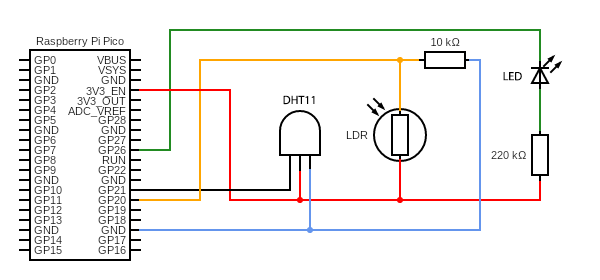
\includegraphics[width=\textwidth]{figures/circuit}
    \caption{Chéma pripojenia k doske Raspberry pi pico W \label{schema1}}
\end{figure}

V prípade potreby možno dosku \textit{Raspberry Pi Pico W} zameniť na dosku \textit{ESP32}. Teoreticky by s použitím tejto dosky nemali byť žiadne problémy, ale táto verzia nebola úplne otestovaná.

\subsection{Softvér meteostanice}
Celá logika meteostanice je napísaná v programovacom jazyku \textit{MicroPython} verzie v1.20.0. 

Program projektu sa skladá z niekoľkých súborov:
\begin{itemize}
    \item \verb|start.py| - štartovací súbor celého programu, ktorý obsahuje logiku prechodu z jedného stavu do druhého.
    \item \verb|states.py| - súbor, ktorý obsahuje logiku jednotlivých stavov. 
    \item \verb|helper.py| - pomocné funkcie. 
    \item \verb|settings.py| - súbor pre systémové premenné. 
    \item \verb|data.txt| - súbor vyrovnávacej pamäte na ukladanie neodoslaných údajov.
\end{itemize}
Projekt používa aj knižnicu tretej strany s názvom \verb|umqtt.simple| na pripojenie k \gls{mqtt} brokeru. 

Životný cyklus meteostanice pozostáva zo 4 stavov a je popísaný funkciami v kóde aplikácie.

Konkrétne funkcie:

\begin{itemize}
    \item \verb|init| - v tejto funkcii sa zariadenie pripojí k \textit{WiFi} a \gls{mqtt} a synchronizuje čas. Úspešnosť pripojenia je signalizovaná prostredníctvom \gls{led} diódy. 
    \item \verb|measure| - zariadenie meria vlhkosť, teplotu, úroveň svetla a čas merania. Potom sa údaje prevedú do formátu JSON na ďalší export.
    \item \verb|upload| - zozbierané údaje sa odošlú do \gls{mqtt} brokera. Ak sa zariadenie nemohlo pripojiť k sieti WiFi alebo k brokeru \gls{mqtt}, údaje sa archivujú do súboru data.txt a odošlú sa pri ďalších pokusoch na pripojenie k internetu. 
    \item \verb|sleep_pico| - zariadenie sa prepne do energeticky efektívneho režimu na pridelený čas.
\end{itemize}

Počas školenia študenti dostanú tieto funkcie prázdne a ich úlohou je naprogramovať vyššie uvedenú logiku v rámci týchto funkcií. Učiteľ počas programovania vystupuje ako supervízor a mentor.

\section{Súčasti \gls{iot} brány}
\subsection{Hardvér}
\gls{gw} sa skladá len z jednej časti, konkrétne z mikropočítača \textit{Raspberry Pi 3}. Môžete použiť aj novšiu verziu, konkrétne \textit{Raspberry Pi 4}. 

Zariadenie musí byť pripojené k internetu prostredníctvom káblového pripojenia alebo cez adaptér \textit{WiFi}. 

\subsection{Softvér}
\gls{gw} je založený na technológii Mosquito a má nainštalovaný Docker a \textit{Node Red}. Podrobnejšiu konfiguráciu systému nájdete v bakalárskej práci \textit{Otvorený \gls{iot} Lab pre stredné školy}\cite{bookSimon}. 

V tejto fáze vývoja projektu študenti používajú programovací jazyk \textit{Node Red} na analýzu a vizualizáciu údajov odosielaných z meteorologickej stanice. Na obrázku \ref{nodeVisual1} je znázornený príklad takejto vizualizácie.

\begin{figure}[!ht]
    \centering
    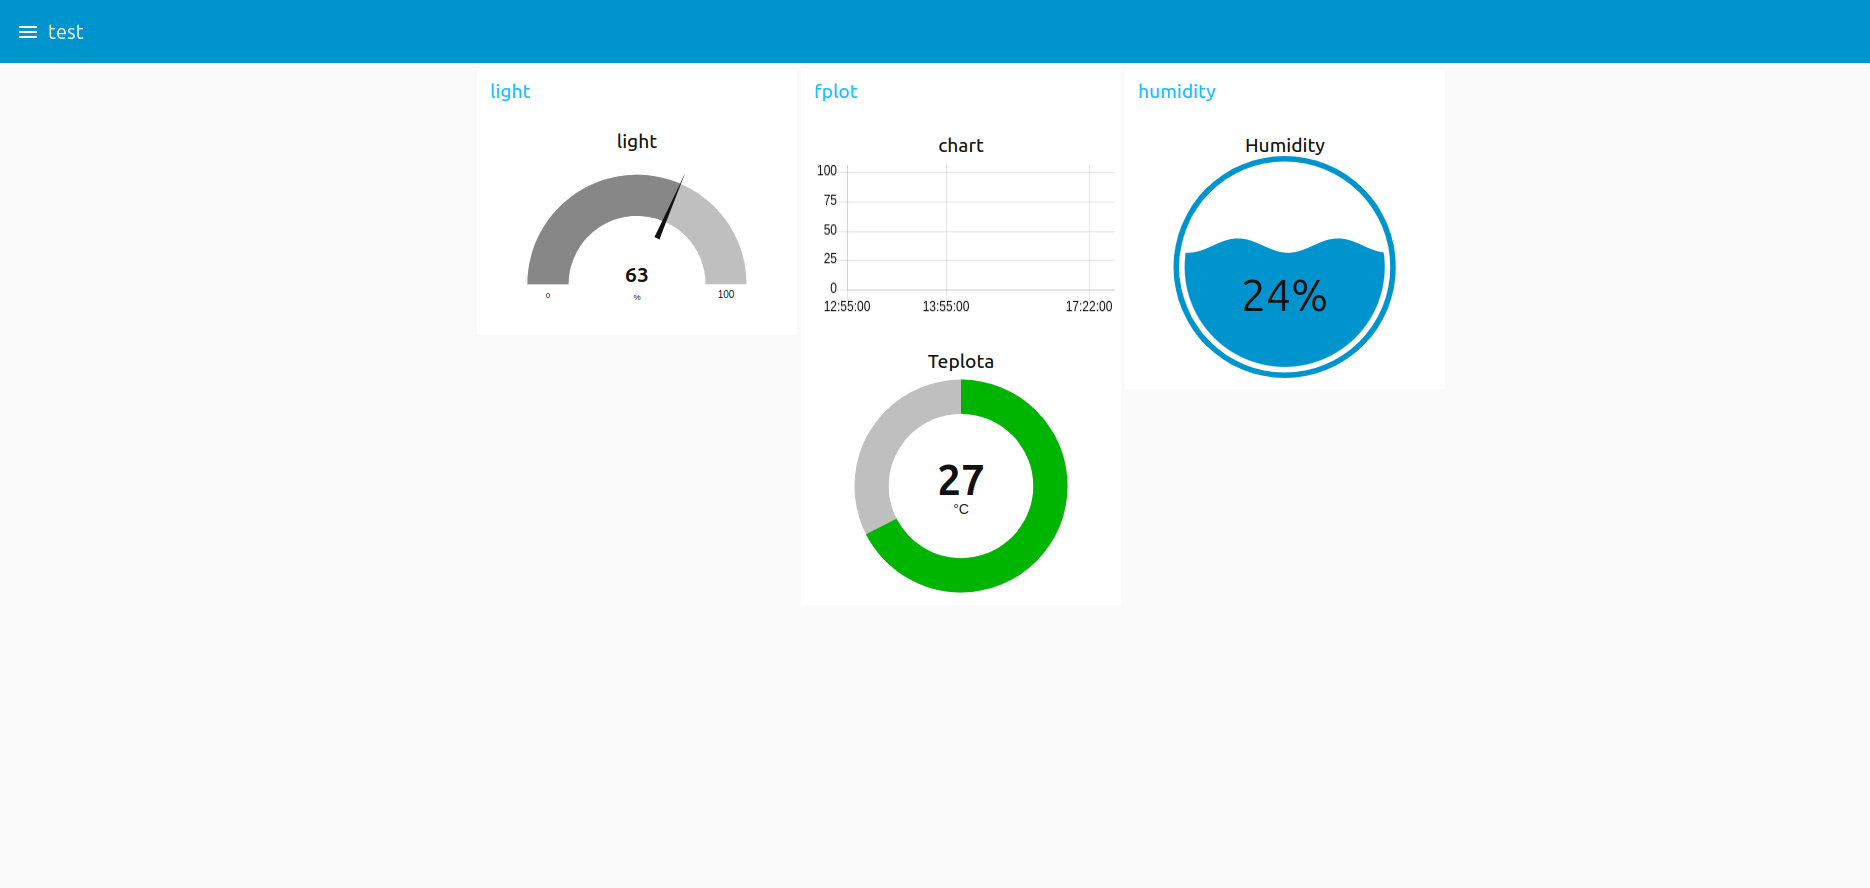
\includegraphics[width=\textwidth]{figures/node_obr}
    \caption{Vizualizácia aplikácie vytvorenej na \textit{Node Red}. \label{nodeVisual1}}
\end{figure}

\subsection{Alternatívny postup}
Vo všeobecnosti môže ako brána slúžiť akýkoľvek iný počítač (napr. počítač učiteľa), pokiaľ je na ňom nakonfigurovaný \gls{mqtt} broker (napr. \textit{Hivemq} alebo \textit{Mosquito}) a nainštalovaný \textit{Docker} a \textit{Node Red}.
